\expandafter\newcommand\csname databLRmetrictab\endcsname{
\begin{table}[H]
\begin{tabular}
{| 
 p{\dimexpr0.2\textwidth-2\tabcolsep-\arrayrulewidth\relax}| 
 p{\dimexpr0.2\textwidth-2\tabcolsep-\arrayrulewidth\relax}| 
 p{\dimexpr0.2\textwidth-2\tabcolsep-\arrayrulewidth\relax}| 
 p{\dimexpr0.2\textwidth-2\tabcolsep-\arrayrulewidth\relax}| 
 p{\dimexpr0.2\textwidth-2\tabcolsep-\arrayrulewidth\relax}| 
}\hline 
\textbf{} &\textbf{f1-score} &\textbf{precision} &\textbf{recall} &\textbf{support} \\ \hline 
CONFIRMED &0.821 &0.843 &0.801 &241.0 \\ \hline 
FALSE POSITIVE &0.926 &0.916 &0.936 &561.0 \\ \hline 
accuracy &0.895 &0.895 &0.895 &0.895 \\ \hline 
macro avg &0.874 &0.88 &0.868 &802.0 \\ \hline 
weighted avg &0.894 &0.894 &0.895 &802.0 \\ \hline 
\end{tabular} 
\end{table}
}
\begin{figure}[H]
                \centering
                \begin{subfigure}{.49\textwidth}
                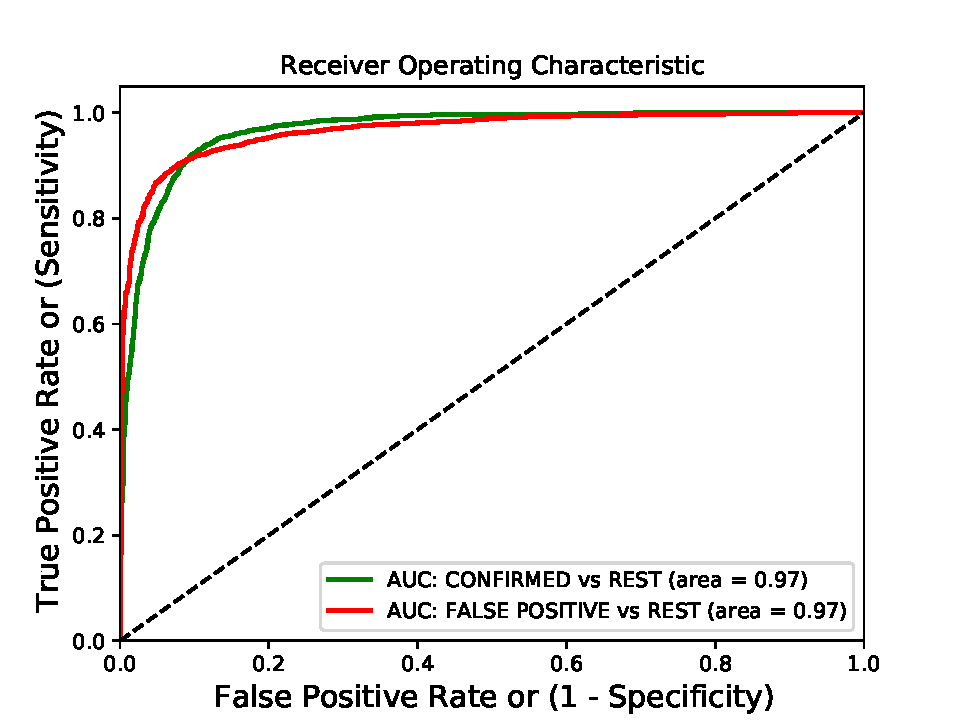
\includegraphics[width = 1\textwidth]{data/bLR_overfit_roc.pdf}
                \end{subfigure}
                \begin{subfigure}{.49\textwidth}
                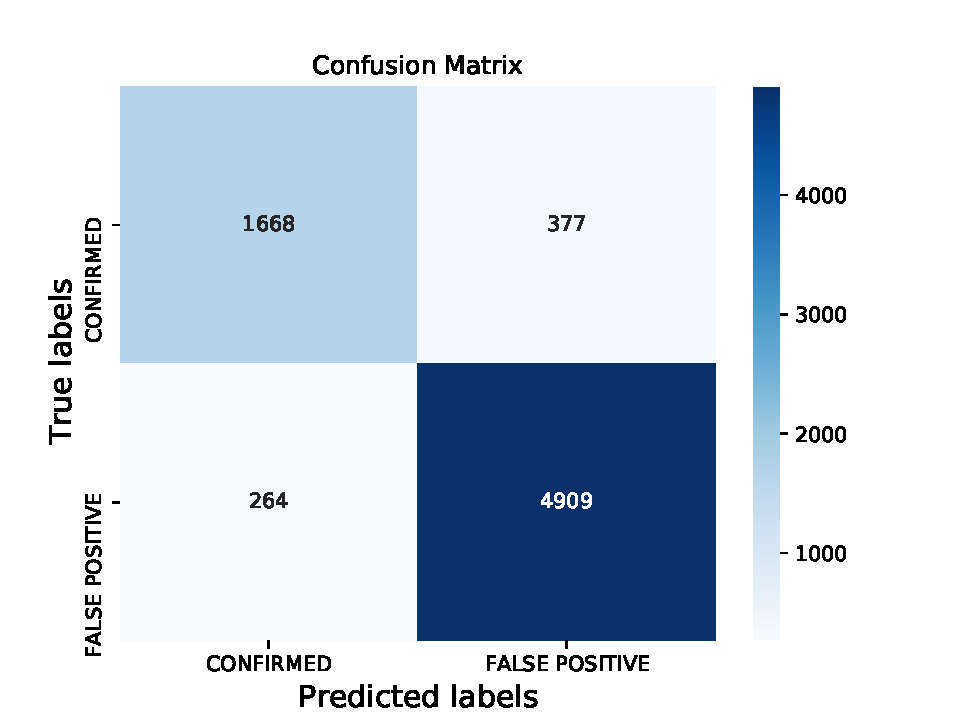
\includegraphics[width = 1\textwidth]{data/bLR_overfit_cm.pdf}
                \end{subfigure}
                \begin{subfigure}{.49\textwidth}
                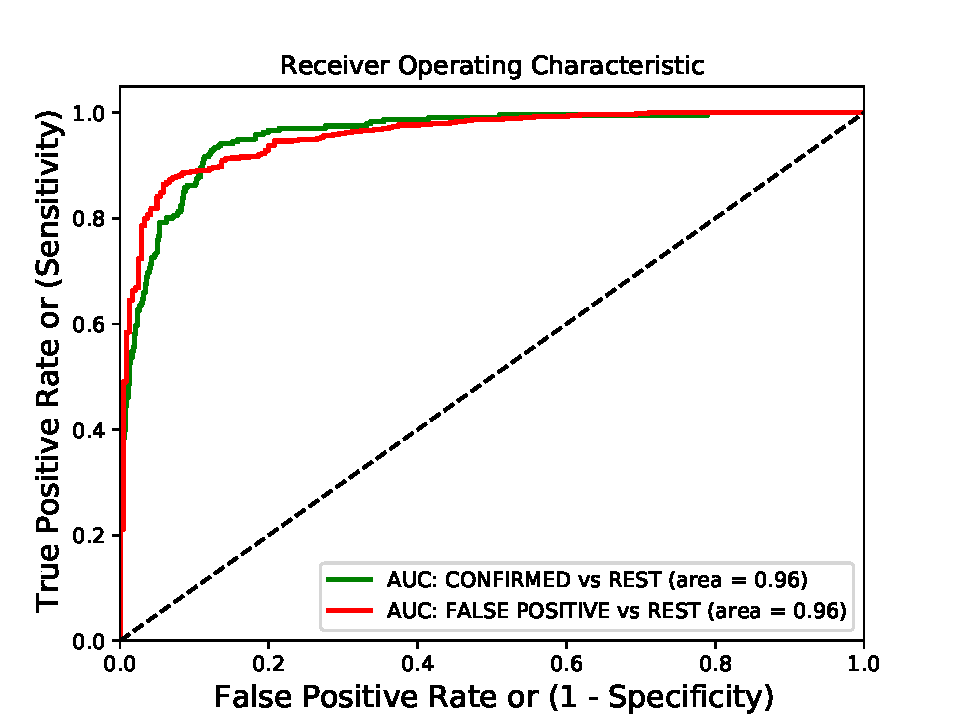
\includegraphics[width = 1\textwidth]{data/bLR_roc.pdf}
                \end{subfigure}
                \begin{subfigure}{.49\textwidth}
                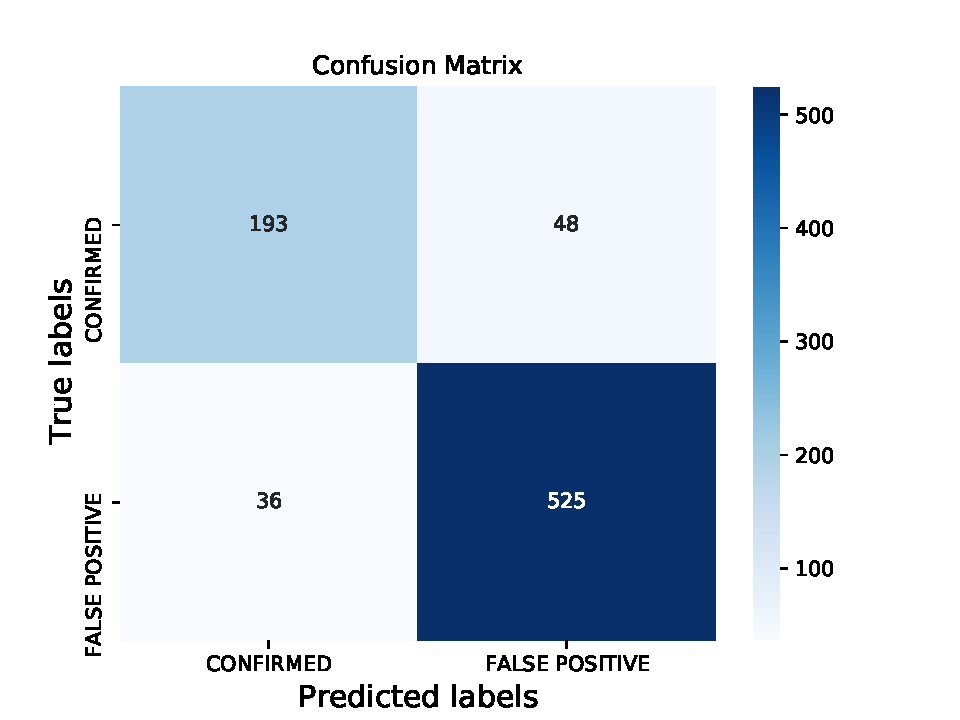
\includegraphics[width = 1\textwidth]{data/bLR_cm.pdf}
                \end{subfigure}
                \begin{subfigure}{1\textwidth}
                \csname databLRmetrictab\endcsname
                \end{subfigure}
                \caption{bLR: Top Row: overfit test. Middle and bottom row test data}
                \label{fig:data/bLR_roc}
                \end{figure}